\documentclass[12pt]{report}
\usepackage{graphicx}
\usepackage{afterpage}
\usepackage{sectsty}  
\usepackage{mathptmx} 
\usepackage{multicol}
\usepackage{titlesec}
\usepackage[a4paper,left=1.5in,right=1.0in,top=24mm,bottom=1.25in]{geometry}
\linespread{1.5} 
\usepackage{etoolbox}% http://ctan.org/pkg/etoolbox

\makeatletter
% \patchcmd{<cmd>}{<search>}{<replace>}{<success>}{<failure>}
\patchcmd{\@makechapterhead}{\huge}{\large}{}{}% for \chapter
\patchcmd{\@makechapterhead}{\Huge}{\large}{}{}% for \chapter
\patchcmd{\@makeschapterhead}{\Huge}{\large}{}{}% for \chapter*
\makeatother




\chapterfont{\centering}
\sectionfont{\fontsize{12}{15}}


\titleformat*{\section}{\normalfont\fontsize{12}{15}\bfseries }
\titleformat*{\subsection}{\normalfont\fontsize{12}{15}\selectfont}

\graphicspath{ {images/} }
% Title Page
\title{}
\author{}


\begin{document}
	

\begin{abstract}
	            Big Data analytics plays a key role through reducing the data size and complexity in Big Data applications. Visualization is an important approach to helping Big Data get a complete view of data and discover data values. Big Data analytics and visualization should be integrated seamlessly so that they work best in Big Data applications. Conventional data visualization methods as well as the extension of some conventional methods to Big Data applications are introduced in this paper. This report presents the recent methods used in Bigdata visualization ,it's applications , technological progress and challenges involved.
\end{abstract}

\tableofcontents
\listoffigures

\chapter{INTRODUCTION}
\section {Data Visualization Market}
Data visualization is representing data in some systematic form including attributes and variables for the unit of information. Visualization-based data discovery methods allow business users to mash up disparate data sources to create custom analytical views. Advanced analytics can be integrated in the methods to support creation of interactive and animated graphics on desktops,laptops, or mobile devices such as tablets and smart phones. Benefits of data visualization according to the respondent percentages of a survey includes improved decision making,better ad-hoc data analysis,improved collaboration,provide self service capability to end users,time savings etc.
\section{The Rise Of Data Visualization}
Data illustration techniques have been in use since as early as 6200 BC, when the oldest known map was drawn. However, it was not until the eighteenth century when data visualizations went beyond mapping and more abstract measures were introduced, including the ever-popular pie and bar charts.The nineteenth century saw the creation of what many have argued to be the world’s best data visualization: Charles Joseph Minard’s 1869 visualization titled Napoleon’s March, which depicts the movement and losses of Napoleon’s army as it invaded Russia in 1812.After 1975, we witnessed the most rapid advancements in data visualization, which stemmed from the development of software and computer systems.\par 
Data visualizations moved beyond pie and bar charts, and more complex formats began to appear and aid us in processing information. For example, through the use of mind maps, our thought patterns can now be visually organized. Apps like Flipboard and Newsmap have completely reinvented the display of news, while tag clouds have provided another way to discover and search for information. And through network graphs, we can now uncover the connectivity between any number of entities, be they our own social circles, groups of companies or globally dispersed cities.
         

\chapter{BIG DATA ANALYTICS}
BigData, according to Wikipedia (Sep 2015), is “the term for a collection of data set so large and d complex that it becomes difficult to process using on n-hand database management tools or traditional d data processing applications”. The data-sets not only contain structured databases, but also include unstructured d databases such as social media data or GPS (Global Positioning System) data.
\par BigData comes from everywhere influence our life, and so is too big, too complex and moves too fast. For example, posting pictures and writing comments on Facebook; uploading and watching videos on YouTube; sending and receiving messages through smart phones; sending voice messages through Whatspapp all count as BigData. To analyse BigData, new analytical methods have to be developed to feed business, government and organization needs.
\par Distributed computing and  parallel processing techniques are widely used in industry for BigData applications. Hadoop (High-availability distributed object oriented platform), the most  popular open-source platform for reliable, scalable, distributed computing, is often referred to by BigData researchers. Two main core frameworks in Hadoop: Hadoop Distributed File System (HDFS) and MapReduce, have being deployed in industries for the management of cluster distributed data centers such as Facebook, Google, Yahoo, Amazon. com, eBay and Twitter (hadoop.appache.org).
\section{3V’s Model And New V’s for Bigdata}
According to Gartner 3Vs definition[3], Volume, velocity and variety to characterize the concept of Big Data.
\subsection{Volume}
90\% of all data ever created was created in the past 2 years. From now on, the amount of data in the world will double every two years. By 2020, we will have 50 times the amount of data as that we had in 2011. The sheer volume of the data is enormous and a very large contributor to the ever expanding digital universe is the Internet of Things with sensors all over the world in all devices creating data every second. The era of a trillion sensors is upon us.
If we look at airplanes they generate approximately 2,5 billion Terabyte of data each year from the sensors installed in the engines.  Self-driving cars will generate 2 Petabyte of data every year. Also the agricultural industry generates massive amounts of data with sensors installed in tractors. Shell uses super-sensitive sensors to find additional oil in wells and if they install these sensors at all 10.000 wells they will collect approximately 10 ExaByte of data annually. That again is absolutely nothing if we compare it to the Square Kilometer Array Telescope that will generate 1 Exabyte of data per day.
\par In the past, the creation of so much data would have caused serious problems. Nowadays, Bigdata technologies allows us  to manipulate such a huge volume of data
\subsection{Velocity}
The Velocity is the speed at which the data is created, stored, analysed and visualized. In the past, when batch processing was common practice, it was normal to receive an update from the database every night or even every week. Computers and servers required substantial time to process the data and update the databases. In the big data era, data is created in realtime or near real-time. With the availability of Internet connected devices, wireless or wired, machines and devices can pass-on their data the moment it is created.
\par
The speed at which data is created currently is almost unimaginable: Every minute we upload 100 hours of video on YouTube. In addition, every minute over 200 million emails are sent, around 20 million photos are viewed and 30.000 uploaded on Flickr, almost 300.000 tweets are sent and almost 2,5 million queries on Google are performed.
\subsection{Variety}
In the past, all data that was created was structured data, it neatly fitted in columns and rows but those days are over. Nowadays, 90\% of the data that is generated by organisation is unstructured data. Data today comes in many different formats: structured data, semi-structured data, unstructured data and even complex structured data. The wide variety of data requires a different approach as well as different techniques to store all raw data.
\par
There are many different types of data and each of those types of data require different types of analysis or different tools to use. Social media like Facebook posts or Tweets can give different insights, such as sentiment analysis on your brand, while sensory data will give you information about how a product is used and what the mistakes are.

\section{The Four Additional V’s}
Now that the context is set regarding the traditional V’s, let’s see which other V’s are important for organisations to keep in mind when they develop a big data strategy.
\subsection{Veracity}
Having a lot of data in different volumes coming in at high speed is worthless if that data is incorrect. Incorrect data can cause a lot of problems for organisations as well as for consumers. Therefore, organisations need to ensure that the data is correct as well as the analysis performed on the data are correct. Especially in automated decision-making, where no human is involved anymore, you need to be sure that both the data and the analyses are correct.
\par
IBM coined Veracity as the fourth V, which represents the unreliability inherent in some sources of data. For example, customer sentiments in social media are uncertain in nature, since they entail human judgment. Yet they contain valuable information. Thus the need to deal with imprecise and uncertain data is another facet of big data, which is addressed using tools and analytics developed for management and mining of uncertain data.
\subsection{Variability}
Big data is extremely variable. Brian Hopkins, a Forrester principal analyst, defines variability as the “variance in meaning, in lexicon”. He refers to the supercomputer Watson who won Jeopardy. The supercomputer had to “dissect an answer into its meaning and to figure out what the right question was”. That is extremely difficult because words have different meanings an all depends on the context. For the right answer, Watson had to understand the context.
\par
Variability means that the meaning is changing (rapidly). In (almost) the same tweets a word can have a totally different meaning. In order to perform a proper sentiment analyses, algorithms need to be able to understand the context and be able to decipher the exact meaning of a word in that context. This is still very difficult. SAS introduced Variability as additional dimensions of big data. Variability refers to the variation in the data flow rates. Often, big data velocity is not consistent and has periodic peaks and troughs.This imposes a critical challenge: the need to connect, match, cleanse and transform data received from different sources.
\subsection{Value}
All that available data will create a lot of value for organisations, societies and consumers. Big data means big business and every industry will reap the benefits from big data. It is estimated that potential annual value of big data to the US Health Care is \$300 billion, more than double the total annual health care spending of Spain. They also mention that big data has a potential annual value of € 250 billion to the Europe’s public sector administration. Even more, in their well-regarded report from 2011, they state that the potential annual consumer surplus from using personal location data globally can be up to \$ 600 billion in 2020. That is a lot of value.
\par
Of course, data in itself is not valuable at all. The value is in the analyses done on that data and how the data is turned into information and eventually turning it into knowledge. The value is in how organisations will use that data and turn their organisation into an information-centric company that relies  on insights derived from data analyses for their decision-making.
\subsection{Visualization}
This is the hard part of big data. Making all that vast amount of data comprehensible in a manner that is easy to understand and read. With the right analyses and visualizations, raw data can be put to use otherwise raw data remains essentially useless. Visualization of course do not mean ordinary graphs or pie charts. They mean complex graphs that can include many variables of data while still remaining understandable and readable.
\par
Visualizing might not be the most technological difficult part; it sure is the most challenging part. Telling a complex story in a graph is very difficult but also extremely crucial. Luckily there are more and more big data start-ups appearing that focus on this aspect and in the end, visualizations will make the difference.



\chapter{DATA VISUALIZATION METHODS}

A picture is worth a thousand words – especially when you are trying to understand and gain insights from data. It is particularly relevant when you are trying to find relationships among hundreds, or even thousands, of variables to determine their relative importance.
\section{Conventional Data Visualization Methods}
Many conventional data visualization methods are often used. They are: table, histogram, scatter plot, line chart, bar chart, pie chart, area chart, flow chart, bubble chart, time line, Venn diagram, data flow diagram, and entity relationship diagram, etc. In addition, some data visualization methods have been used although they are less known compared the above methods. The additional methods are: parallel coordinates, treemap, cone tree, and semantic network, etc.
\par
There are many conventional data visualization techniques which are focused in this document because these techniques have generic features and common understanding. These data presentation should be beautiful, elegant, descriptive, and interpretable in order to convey message to the reader effectively. There are new developed fascinating methods are introducing, but modern approaches have its own implementation problems and no commonality, so difficult to adopt. Data visualization represents data in the way that simplifies data interpretation and its relationship.
\subsection{Pie Chart}
A pie chart is also called circle graph. Pie chart circle is divided into number of sectors, each circle describe a proportion in a whole quantity. The pie chart control is use to determines the size of data wedge as compare to other data wedges. In pie chart a wedge represents the part of data that has common feature or characteristics. Wedges can be labeled to identify different data points. Most of the time is shown in percentage.
\begin{figure}[h]
	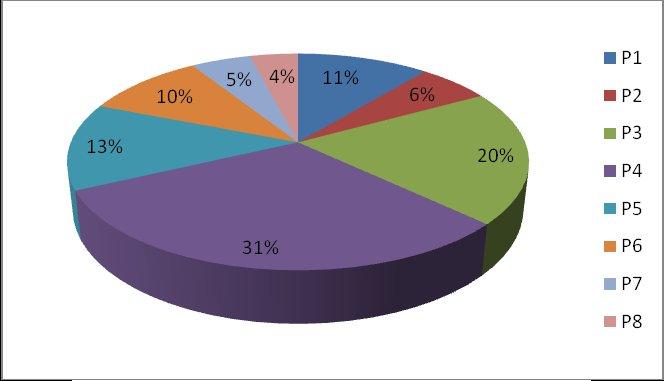
\includegraphics[width=4cm, height=4cm]{piechart}
	\centering
	\caption{Standard Pie Chart}
\end{figure}.
\subsection{Bar Chart}
One of the most commonly use data visualization method is bar chart, it is also called Bar Graph(also called Column chart). Bar chart is most of the time use for discrete data not for continuous data. Bar Chart control has been use to represent data in horizontal bars, the vertical length of the bar represent the values. Bar chart is use to represent a single data series and related data points are group in one series. For example monthly salaries, it can be mutli bar graph i.e. percentage increase per month as shown in the following figure.

\begin{figure}[h]
	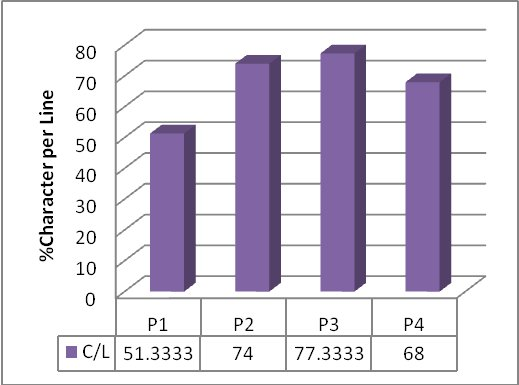
\includegraphics[width=4cm, height=4cm]{barchart}
	\centering
	\caption{Bar Chart}
\end{figure}
\subsection{Line Chart}
Line chart is common well known graph in many fields, also label as line graph. It is a graph which is use to display information in connected points. These points are connected through continuous or straight line. Line graph is the extension of Scatter plot. Data points can be represented by icons or symbols, or can also draw simple line without icons
\begin{figure}[h]
	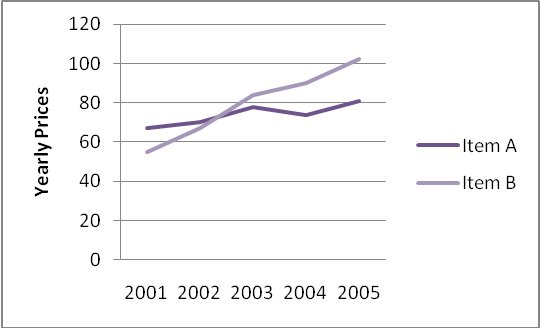
\includegraphics[width=4cm, height=4cm]{linechart}
	\centering
	\caption{Line Chart}
\end{figure}
\subsection{Area Chart}
Area chart is also called area graph, use to display quantitative data graphically. Area chart control is use represent data in bounded area. The bounded area is based on the line graph, the line is generated and the area below is shaded with colors,different texture and hatching, which produce area graph.
\begin{figure}[h]
	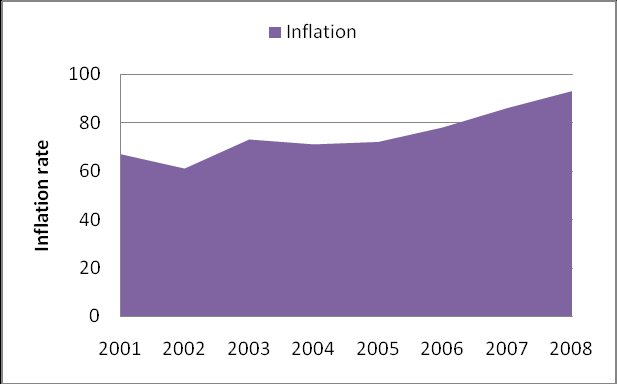
\includegraphics[width=4cm, height=4cm]{areachart}
	\centering
	\caption{Area Chart}
\end{figure}
\subsection{Scatter Plot}
Scatter Plot is also known as plot, plot chart, scatter chart, scattergram, scatter diagram or scatter graph. Scatter plot is graphical display of set of data in Cartesian coordinate, shows the relationship between two variables, one variable represent horizontal distance (independent variable) and second variable vertical distance (dependent variable) of data point from the coordinate axis. Scatter plot shows the how strong the relationship are between the variables, and determines whether their exit any outlier in the data or not. It is use to look how the data is dispersed.
\begin{figure}[h]
	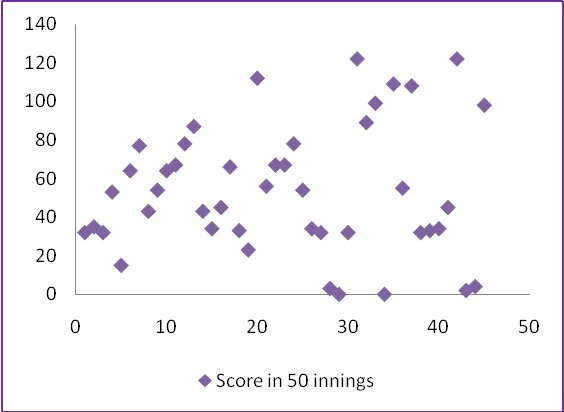
\includegraphics[width=4cm, height=4cm]{scatterplot}
	\centering
	\caption{Scatter Plot Diagram}
\end{figure}

\section{Interactive Visualization}
The users are interested in the abstract data about which they have desire to understand, the user don’t have sufficient pre knowledge about that data. Hence for the exploration, analysis, and for the representation of data or information visualization interactive techniques are exceptionally momentous. The challenge in information visualization is to provide data visually in order to the user effectively understand the information for which the user is looking for, for this purpose provide interaction mechanism that make is possible to manipulate visualization effectively and effortlessly as probable. Users can interact with interfaces or visualization in different ways by means of mouse over, single click, double click, or can add multiple interactive options by mouse right button click. There are many interactive techniques available to interact with charts or graphical representation to understand the drill down details. Card et al introduce the interactive mechanism of visualization in 1999.
\par
Interactive visualization can be performed through approaches such as zooming (zoom in and zoom out), overview and detail, zoom and pan, and focus and context or fish eye. The steps for interactive visualization are as follows:
\subsection{Selecting}
One of the most important and fundamental requirements in visualization is interactive selection of data entities or subset or part of whole data or whole data set, that is of interest to the user. This is useful to view detail information about the selected entities, highlight entities that are covered or hidden, cluster entities that are related and extracting entities that may be use in future.
\subsection{Linking}
Linking and brushing are the most common form of linking. Linking is useful to relate information among multiple views. Information can be mapped differently to different views to reveal or expose different perspectives (viewpoint) or different portions of the information. On the bases of selection criteria the user can select entities in one structure, which then shows the distribution the selected entities in another structure.
\subsection{Filtering}
Filtering enables users to dynamically adjust amount of information to display, means to decrease or increase information quantity that need to display, and focus on information of interest. For this purpose need some dynamic query values to manipulate, in this regard visual widgets can play vital role e.g. slider can be use in different ranges, field box can be use to put attribute value in specified range etc. these widgets enables one from the current query parameters and enables to quickly adjust query parameters and instantaneously view filtered results in the visualization in real time.
\subsection{Rearranging or Remapping}
As a single mapping or plotting visual form of information may be not enough, so the users must empower to customize mapping among many maps. To enable users to customize maps by its own choice provide the way to better understand the information. As the spatial layout is the most important visual mapping, rearranging the spatial layout of the information is the most effective for producing different insights
\begin{figure}[h]
	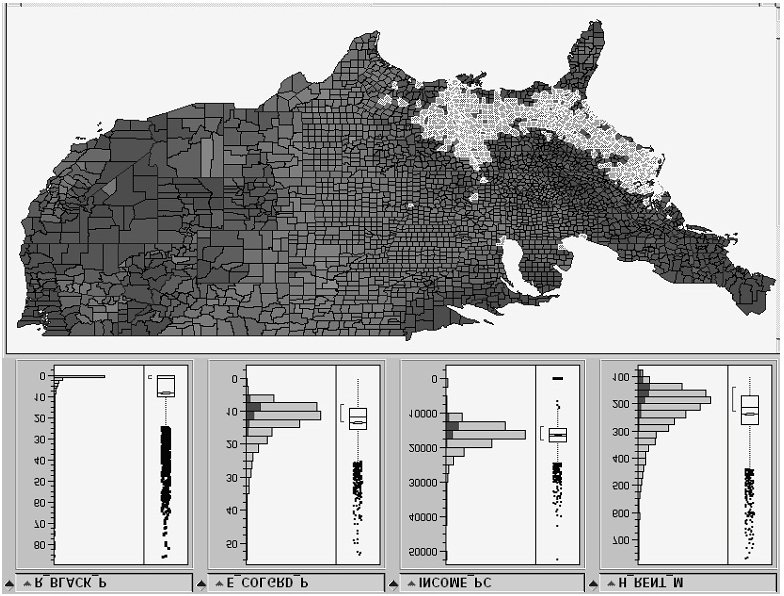
\includegraphics[width=\textwidth, height=8cm]{interactivebrushing}
	\centering
	\caption{Interactive brushing and linking between histogram plots (top) and geographic map (bottom) of datasets}
\end{figure}
\section{Data Visualization Tools}
Following are the most awesome data visualization tools available on the web
\begin{itemize}
	\item Dygraph
	\item ZingCharts
	\item InstantAtlas
	\item Timeline
	\item Exhibit
	\item Modest Maps
	\item Leaflet
	\item WolframAlpha
	\item Visual.ly
	\item VisualizeFree
	\item Better World Flux
	\item Fusion Charts
	\item jqPlot
	\item Dipity
	\item Many Eyes
	\item D3.js
	\item jpGraphs
	\item HighCharts
	\item Google Charts
	\item CrossFilter
\end{itemize}



\chapter{BIG DATA VISUALIZATION AND CHALLENGES}
Visualization is an essential tool for making sense of big data.It provides a far richer view of big data than can be obtained  from tables and statistics alone. However, the key to effective analysis of big data is the integration of visualization into analytics tools so that all kinds of users can interpret big data from a wide range of sources — click streams, social media, log files, videos and more.
\par
Online marketplace eBay, have hundreds of million active users and billions of goods sold each month, and they generate a lot of data. To make all that data understandable, eBay turned to Big Data visualization tool: Tableau, which has capability to transform large, complex data sets into intuitive pictures. The results are also inter-active. Based on them, eBay employees can visualize search relevance and quality to monitor the latest customer feedback and conduct sentiment analysis.
\section{Challenges in Big Data Visualization}
For Big Data applications, it is particularly difficult to conduct data visualization because of the large size and high dimension of Big Data. However, current Big Data visualization tools mostly have poor performances in functionalities, scalability and response time. What we need to do is rethinking the way we visualize Big Data, not like the way we adopt before. For example, the history mechanisms for information visualization also are data-intensive and need more efficient approaches. Uncertainty can lead to a great challenge to effective uncertainty-aware visualization and arise in any stage of a visual analytics process. New framework for modeling uncertainty and characterizing the evolution of the uncertainty information are highly necessary through analytical processes.
\par Major challenges in visual analytics are
\subsection{Scalability}
Scalability represents the scalability of visual representations.A visual analytics tool which can be used for lower dimensions of data may not be appropriate for visualizing higher dimensions of data.Since Bigdata applications are involving high dimensions of data we need tools that can operate on these data quickly and effectively.
\par 
Perceptual and interactive scalability are also challenges of big data visualization. Visualizing every data point can lead to over-plotting and may overwhelm users’ perceptual and cognitive capacities; reducing the data through sampling or filtering can elide interesting structures or outliers. Querying large data stores can result in high latency, disrupting fluent interaction
\par 
Scalability of the visualization tool should answer the following questions if it is considered scalable.
\begin{itemize}
	\item How to run queries on distributed systems to explore big data sets?
	\item How to visualize a million multi-variate items on a screen?
	\item How to lower the time needed to run a clustering algorithm on xGbytes?
	\item How to design an interactive user interface loading big data in < 1 sec?
\end{itemize}
\subsection{Dynamics}
Visualization tool should be answer the following questions if it is considered to be dynamic.
\begin{itemize}
	\item How to aggregate data streams?
	\item How to visualize a continuously changing data structure?
	\item How to adapt clustering algorithms to consider dynamic data?
	\item How to design an interactive user interface continuously fed by data?
\end{itemize}
\subsection{Need Of Massive Parallelization}
Due to increasing data sizes and the emergence of the Big Data problem, the need for massive parallelization is a driving visualization research challenge. Supercomputing simulations regularly generate massive data sets with billions of data points per time step. Parallelization is an effective way of dealing with such data: there is more memory for storing data, there is more compute power for executing algorithms, and there is often more I/O bandwidth for reading data. The basic challenge for parallel visualization algorithms is to decompose the problem into independent tasks that can be run concurrently on all of the processing elements (i.e., the instances of the program), thus avoiding idle time.
\par 
Data parallelism is the dominant technique; data sets are decomposed into pieces and the pieces are partitioned over the processing elements. This approach has been shown to be highly scalable with results for hundreds of thousands of processing elements in research prototypes and tens of thousands of processing elements in production software .The role of visualization software, with respect to parallelization, is to provide a framework that shields algorithm developers from complexity.
\subsection{Application Architecture and Data Management}
Application architecture refers to the system design of visualization software. Data management for visualization must provide visualization techniques that integrate into the data life cycle. Although these two topics are distinct, they are treated together here, since emerging data management needs will drive application architecture. Traditionally, data management has not been a pressing concern for visualization software. Data, whether observed or simulated, was stored in the file system for processing;visualization software simply read whatever data it needed from files whenever it needed it. However, increases in data size, observed and simulated, as well as diversity of data sources, mandate new approaches in data management. 
\par
Application architectures exist to solve the simplest use model: “have data, want a picture," where the application architecture serves as a black box that consumes data and produces imagery with user-selected methods and parameters.Twenty-five years ago, the architecture for most visualization applications was a single binary that read from the local file system and produced images using local graphics. A little over a decade ago, scientific visualization applications for large data shifted to a client-server design where data was processed by a remote parallel server, producing geometry that was rendered by a local client. Today, application architectures for visualization frequently involve web clients and remote data access. In short, application architectures evolve to meet evolving data management needs.
\section{Potential Solutions}
The potential solutions of the common problems in big data visualization is presented in following section.
\subsection{Meeting the Need for Speed}
Meeting the need for speed In today’s hyper-competitive business environment, companies not only have to find and analyze the relevant data they need, they must find it quickly. Visualization helps organizations perform analyses and make decisions much more rapidly, but the challenge is going through the sheer volumes of data and accessing the level of detail needed, all at a high speed. The challenge only grows as the degree of granularity increases. One possible solution is hardware. Some vendors are using increased memory and powerful parallel processing to crunch large volumes of data extremely quickly. Another method is putting data in-memory but using a grid computing approach, where many machines are used to solve a problem.Both approaches allow organizations to explore huge data volumes and gain business insights in near-real time.
\subsection{Dealing with Outliers}
The graphical representations of data made possible by visualization can communicate trends and outliers much faster than tables containing numbers and text.Outliers typically represent about 1 to 5 percent of data, but when you’re working with massive amounts of data, viewing 1 to 5 percent of the data is rather difficult. How do you represent those points without getting into plotting issues? Possible solutions are to remove the outliers from the data (and therefore from the chart) or to create a separate chart for the outliers. You can also bin the results to both view the distribution of data and see the outliers. While outliers may not be representative of the data, they may also reveal previously unseen and potentially valuable insights.
\subsection{Displaying meaningful results}
Plotting points on a graph for analysis becomes difficult when dealing with extremely large amounts of information or a variety of categories of information.For example, if we have 10 billion rows of retail SKU data that we’re trying to compare. The user trying to view 10 billion plots on the screen will have a hard time seeing so many data points. One way to resolve this is to cluster data into a higher-level view where smaller groups of data become visible. By grouping the data together, or “binning,” data can be more effectively visualized.


\chapter{PROGRESS OF BIGDATA VISUALIZATION}
The directions that research is taking for visualizing big data are a mix: both applying existing principles such as “details on demand” at higher levels of scale (for example, providing more levels of drill-down between the overview and the lowest level of granularity) and also coming up with new and specialized visualizations that allow larger quantities of data to be represented intelligibly. And as such tools become more sophisticated and more mainstream.
\section{Big Data Visualization Methodology}
Visualizations should be designed in the era of big data in a way such that visualization tools should provide an overview first, then allow zooming and filtering, and provide deeper details on demand.
\subsection{Overview First}
The most important part of a dashboard is the “overview” section. It’s the first thing a viewer sees in the dashboard, and guides the him or her to other parts of the product for further exploration.
\par
The overview should summarize the overarching story from the entire data set without getting into the minor details. It shouldn’t overload the user with too much data, which is where interactive charts, gauges, and maps serve to reduce data clutter, and bring out the story more powerfully
\par
At the same time it shouldn’t leave out important parts of the story by using just a single pie chart, and hiding all the data a layer deeper. Often, great dashboards use a combination of chart types like the line chart, bar chart, maps, and gauges to give the viewer variety, and clarity when studying the data. The overview section should be carefully planned to highlight the important parts of the story, and give lesser weight to the not-so-critical parts. To do this, you may want to organize the entire section into many sub-sections that are clearly labeled. Of course, the important sections would be placed more prominently than the others.
\subsection{Zoom and Filter}
Since all the data is presented to the user in the overview section, the viewer will want to focus on particular areas of interest. This involves zooming and filtering the data using the dashboard’s interactive features: zooming, scrolling, panning, drill-down, legend, range selector, etc. For example, zooming may be drilling down from global to country-specific data while filtering may be excluding information in a specific time range.
\par 
From a design perspective, designer should aim to provide the user with plenty of control for zooming and filtering data from the overview. This will yield maximum insights and action from the information at hand.
\subsection{Details-on-Demand}
Designer have identified areas of interest from the overview section, and have dug deeper into the data using zooming and filtering, but user still may not have found what he started looking for. 
\par 
A dashboard that excels at giving an overview, and allows extensive zooming and filtering, should go all the way and give the viewer access to the minute details. This would bring them as close as possible to the raw data, and equip them to find what they started looking for. This third layer of data would be less visual, and more text-heavy with a focus on accurate information rather than trends. This way the analyst gets what he or she needs, in a way that drives action.
\section{Big Data Visualization Approach}
Visualization can play an important role in using big data to get a complete view of customers. Relationships are an important aspect of many big data scenarios. Social networks are perhaps the most prominent example and are very difficult to understand in text or tabular format; however, visualization can make emerging network trends and patterns apparent. A cloud-based visualization method was proposed to visualize an inherent relationship of users on social network. The method can intentionally present the users’ social relationship based on the correlation matrix to represent a hierarchical relationship of user nodes of social network. In addition, the method uses Hadoop based on cloud for the distributed parallel processing of visualization, which helps expedite the big data of social network
\par 
Big data visualization can be performed through a number of approaches such as more than one view per representation display, dynamical changes in number of factors, and filtering (dynamic query filters, star-field display, and tight coupling).
\subsection{TreeMap}
It is based on space-filling visualization of hierarchical data.
\begin{figure}[h]
	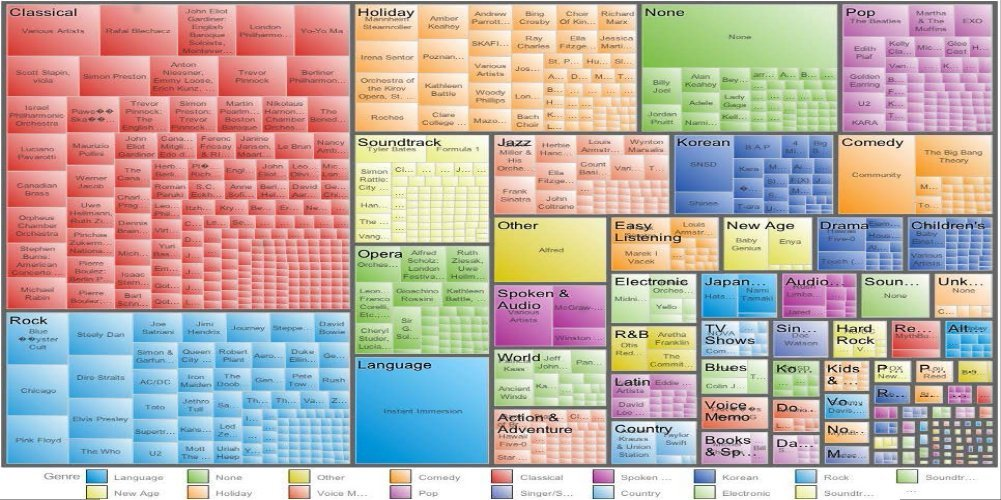
\includegraphics[width=\textwidth, height=8cm]{treemap}
	\centering
	\caption{Treemap}
\end{figure}
\subsection{Parallel Coordinates}
It allows visual analysis to be extended with multiple data factors for different objects.
\begin{figure}[h]
	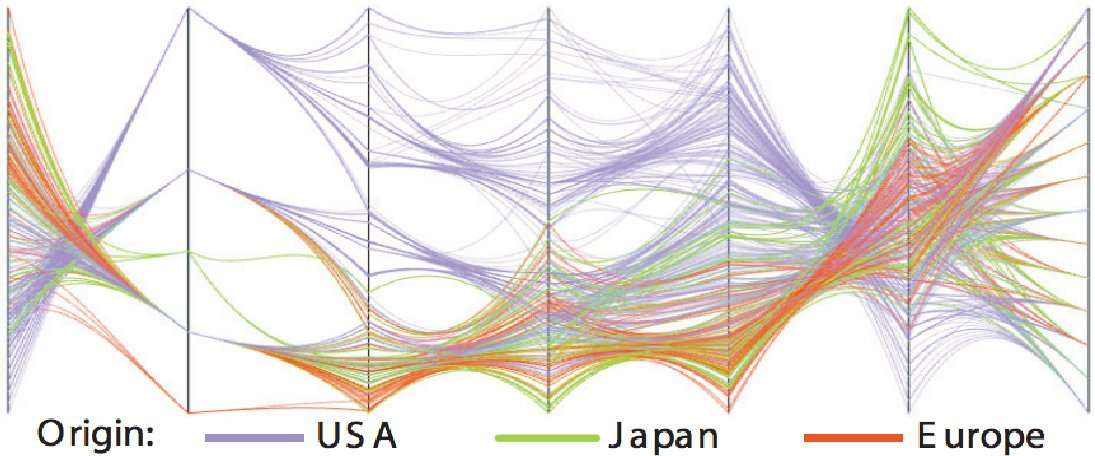
\includegraphics[width=\textwidth, height=5cm]{parallelcoordinates}
	\centering
	\caption{Parallel Coordinates}
\end{figure}
\subsection{Semantic Network}
A semantic network or net is a graph structure for representing knowledge in patterns of 
interconnected nodes and arcs.
\begin{figure}[h]
	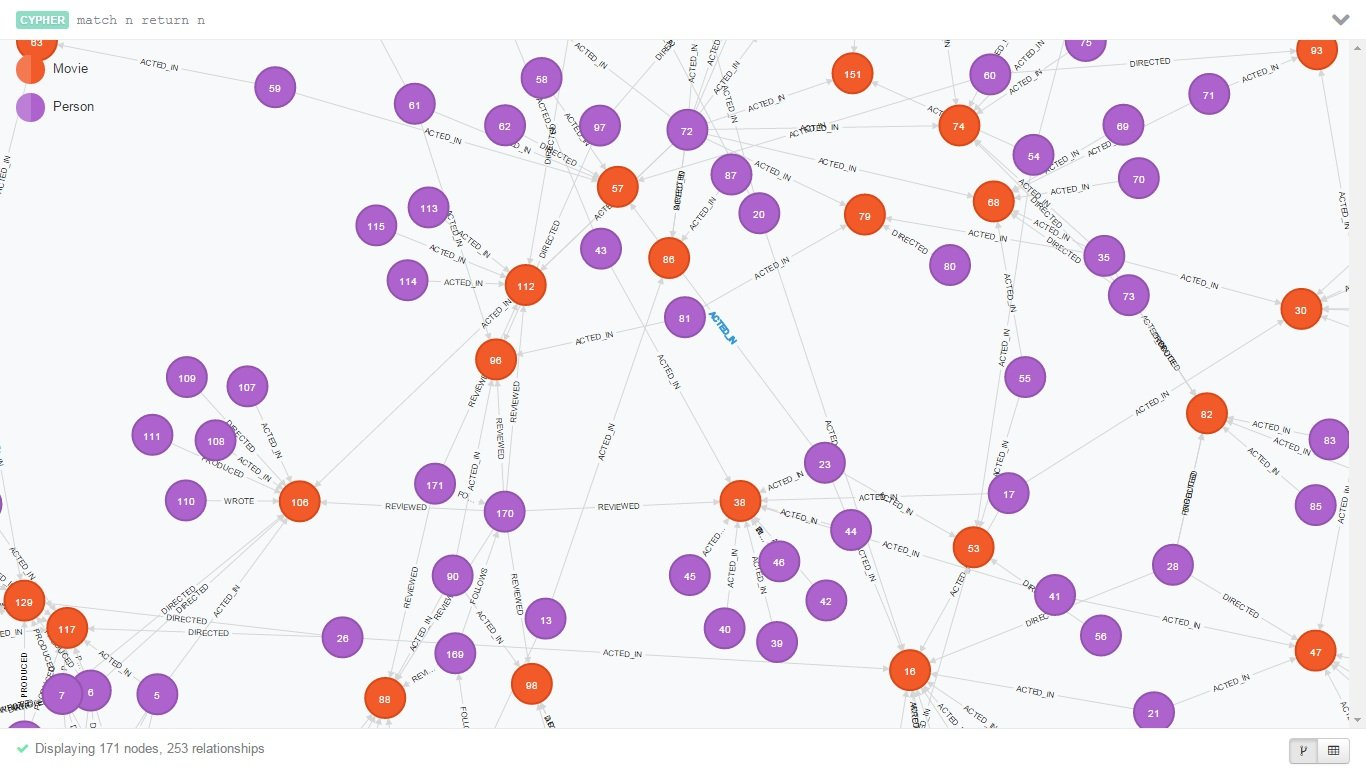
\includegraphics[width=\textwidth, height=6cm]{semanticnetwork}
	\centering
	\caption{Semantic Network}
\end{figure}
\subsection{Sunburst}
It uses tree-map visualization and is converted to polar coordinate system. The main difference is that the variable parameters are not width and height, but a radius and arc length.
\begin{figure}[h]
	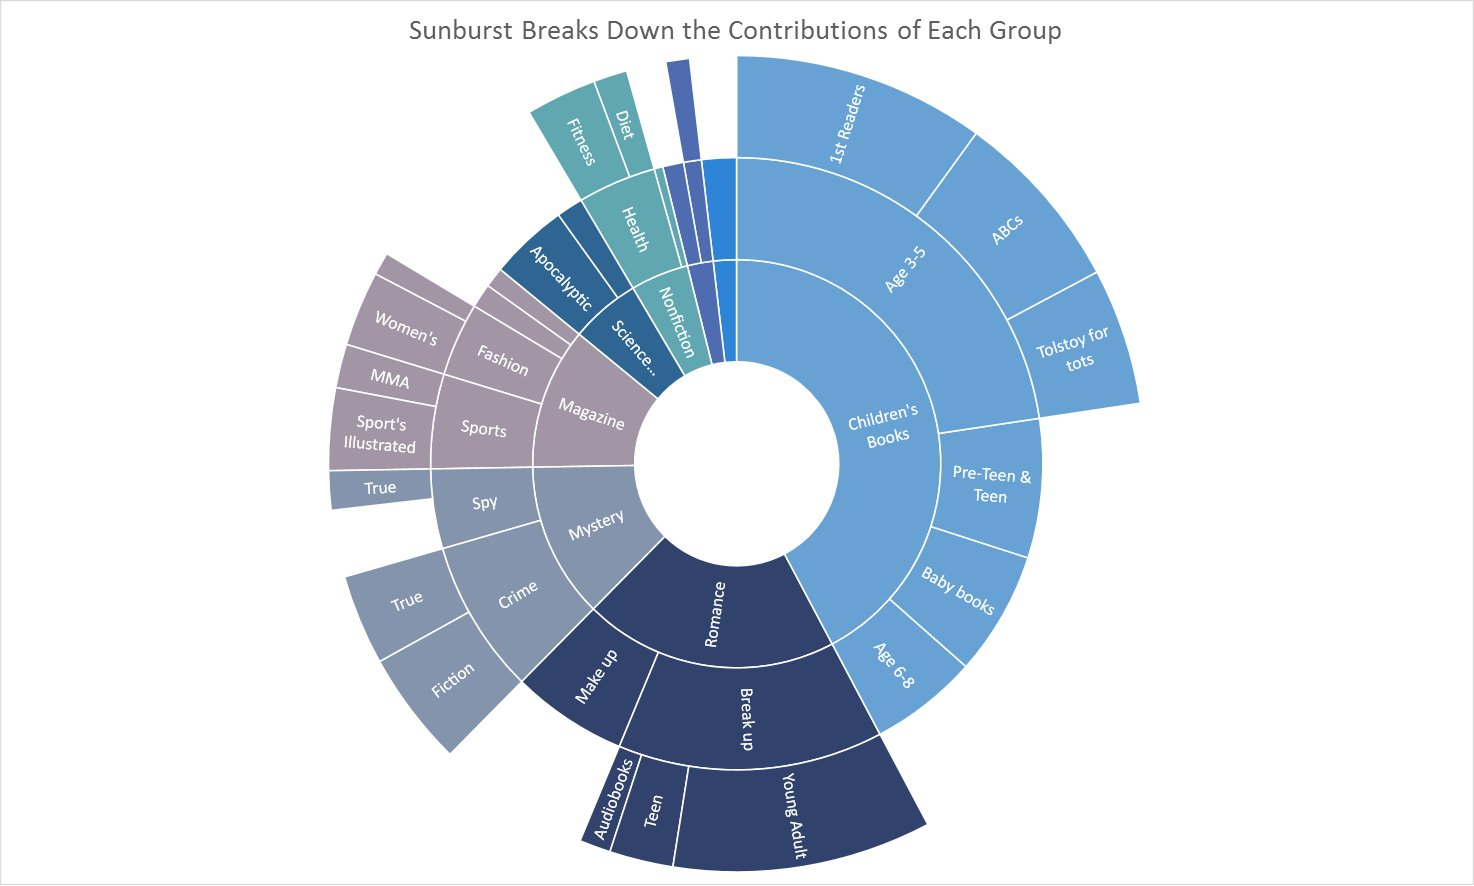
\includegraphics[width=10cm, height=6cm]{sunburst}
	\centering
	\caption{SunBurst Visualization}
\end{figure}
\section{Properties Of Visualization Tools}
Traditional data visualization tools are often inadequate to handle big data. Methods for interactive visualization of big data were presented. First, a design space of scalable visual summaries that use data reduction approaches (such as binned aggregation or sampling) was described to visualize a variety of data types. Methods were then developed for interactive querying (e.g., brushing and linking) among binned plots through a combination of multivariate data tiles and parallel query processing. The developed methods were implemented in imMens, a browser-based visual analysis system that uses WebGL for data processing and rendering on the GPU
\par
Big data processing tools can process ZB (zettabytes) and PB (petabytes) data quite naturally, but they often cannot visualize ZB and PB data. At present, big data processing tools include Hadoop, High Performance Computing and Communications, Storm, Apache Drill, RapidMiner, and Pentaho BI. Data visualization tools include NodeBox, R, Weka, Gephi, Google Chart API, Flot, D3, and Visual.ly, etc. A big data visualization algorithm analysis integrated model based on RHadoop was proposed. The integrated model can process ZB and PB data and show valuable results via visualization. The model is suitable for the design of parallel algorithms for ZB and PB data.
\\
\begin{table}[h!]
\begin{tabular}[h!]{ |p{3cm}||p{3cm}|p{2cm}|p{2.5cm}|}
 \hline
 Method name&Large data volume&Data variety&Data dynamics\\
 \hline
 Treemap&+&-&-\\
 Sunburst&+&-&+\\
 Parallel coordinates&+&+&+\\
 Circular network &+&+&-\\
 Circle packing&+&-&-\\
 \hline
\end{tabular}
\caption{Properties of visualization methods}
\label{table:1}
\end{table}
\section{Virtual Reality Platform for Scientific Data Visualization}
The use of immersive virtual reality (VR) platforms for scientific data visualization has been in the process of exploration including software and inexpensive commodity hardware. These potentially powerful and innovative tools for multi-dimensional data visualization can provide an easy path to collaborative data visualization. Immersion provides benefits beyond traditional “desktop” visualization tools: it results in a better perception of data scape geometry and more intuitive data understanding.
\par
Immersive visualization should become one of the foundations to explore the higher dimensionality and abstraction that are attendant with big data. The intrinsic human pattern recognition (or visual discovery) skills should be maximized through using emerging technologies associated with the immersive VR.
\section{SWOT Analysis Of Current Tools}
The SWOT (Strengths, Weaknesses, Opportunities, and Threats) analysis is a well-known method to ensure that both positive factors and negative factors are identified. A SWOT analysis of the above software tools for big data visualization has been conducted and is shown in table \ref{table:2}. In table \ref{table:2}, Strengths and Opportunities are positive factors; Weaknesses and Threats are negative factors.
\begin{table}[h!]
	\centering
	\begin{tabular}[c]{ |p{6cm}|p{6cm}|}
		\hline
		
		Strengths&Opportunities\\
		\hline
		 With the functions of visualization and interaction for visualizing data.& Immersive visualization with virtual reality (VR) result in a better perception of data scape geometry and more intuitive data understanding.\\
		 \hline
		 Able to visualize a variety of data types&The intrinsic human pattern recognition (or visual discovery) skills
		 could be maximized.\\
		\hline
		\hline
		Weaknesses&Threats\\
		\hline
		There is room to improve in visualizing big data with high velocity or
		the combination of three high Vs (Volume + Velocity + Variety).&Lack adequate visualization in a lot of Big Data applications.\\
		\hline
	\end{tabular}
	\caption{The SWOT analysis of current big data visualization software tools}
	\label{table:2}
\end{table}



\chapter{CONCLUSION}
Visualizations can be static or dynamic. Interactive visualizations often lead to discovery and do a better job than static data tools. Interactive visualizations can help gain great insight from big data. Interactive brushing and linking between visualization approaches and networks or Web-based tools can facilitate the scientific process. Web- based visualization helps get dynamic data timely and keep visualizations up to date.
\par
The extension of some conventional visualization
approaches to handling big data is far from enough in
functions. More new methods and tools of Big Data
visualization should be developed for different Big Data
applications. Advances of Big Data visualization are
presented and a SWOT analysis of current visualization
software tools for big data visualization has been
conducted in this paper. This will help develop new
methods and tools for big data visualization. Big Data
analytics and visualization can be integrated tightly to
work best for Big Data applications. Immersive virtual
reality (VR) is a new and powerful method in handling
high dimensionality and abstraction. It will facilitate Big
Data visualization greatly.

\begin{thebibliography}{25}
	\bibitem{datafloq}
		Datafloq.com, 'Datafloq - The One-Stop Shop for Big Data', 2015. [Online]. Available: https://datafloq.com/read/3vs-sufficient-describe-big-data/166. [Accessed: 27- Oct- 2015].
	\bibitem{bigdata_nextfrontier}	Mckinsey.com, 	'Big data: The next frontier for innovation, competition, and productivity', 2015. [Online]. Available: http://www.mckinsey.com/insights/business\_technology/big\_data \_the\_next\_frontier\_for\_innovation. [Accessed: 27- Oct- 2015].
	\bibitem{garter}
	Stamford, “Gartner Says Solving ‘Big Data’ Challenge Involcves More Than Just Managing
	Volumes of Data”,27,2011,posted on June http://www.gartner.com/newsroom/id/1731 916
	\bibitem{datavisualization} 	
	E.Y. Gorodov and V.V. Gubarev, Analytical Review of Data Visualization Methods in Application to Big Data, Journal of Electrical and Computer Engineering, 013, Article ID 969458, pp.1-7.
\bibitem{khanandkhan} 
M. Khan, S.S. Khan, Data and Information Visualization Methods and Interactive Mechanisms: A Survey, International Journal of Computer Applications, 34(1), 2011, pp. 1-14
\bibitem{intel} 
Intel IT Center, Big Data Visualization: Turning Big Data Into Big
Insights, White Paper, March 2013, pp.1-14.
\bibitem{Sucharitha} 
V. Sucharitha, S.R. Subash and P. Prakash , Visualization of Big
Data: Its Tools and Challenges, International Journal of Applied
Engineering Research, 9(18), 2014, pp. 5277-5290.


\end{thebibliography}


\end{document} 